\section{Modelos de función de base adaptativa}
\label{cap:adaptativa}

\subsection{Introducción}
\label{sec:intro_adap}

Esta sección se refiere a una familia general de modelos que llamaremos modelos de \textbf{función de base adaptativa}, que tienen la forma:
\begin{equation}
    f(x) = w_0 + \sum^K_{k=1} w_k \phi_k(x) \,. 
\end{equation}
A la función $\phi_k(x)$ se le dice la $m$-ésima función de base, la cual variará en función de los datos. Esta familia general de modelos incluye los modelos a estudiar en está sección: árboles, bosques, modelos basados en bagging y boosting, como también las redes neuronales y las sumas generales de modelos \cite{pml1Book}.


\subsection{Árboles}
\label{sec:arbol}

\subsubsection{Motivación con caso regresión}

Antes de definir árboles de manera formal, construiremos una intuición para el caso de regresión. Consideremos una función de una variable. Una manera de aproximar tal función es hacer una interpolación usando funciones constantes. Una primera idea puede ser aproximar la función entera simplemente por su media.

\begin{figure}[h]
	\centering
	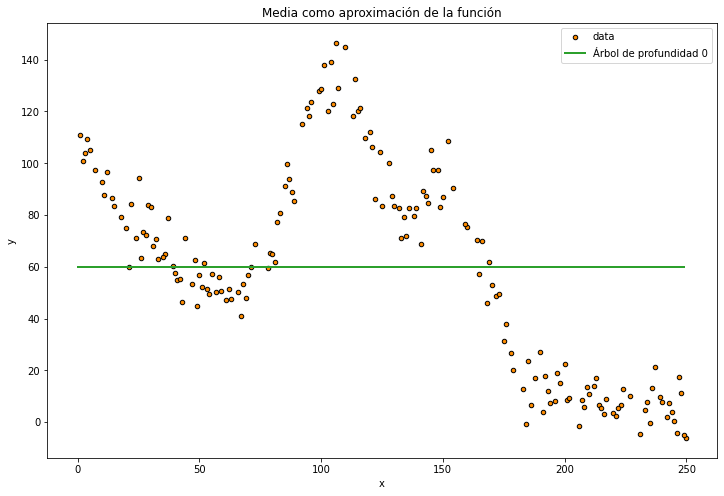
\includegraphics[height=6cm]{img/capN_arbol_trivial.png}\\
	\caption{Aproximación de una función usando su media (árbol trivial no ajustado).}
\end{figure}

Otra manera, más bien voraz, de enfrentar el problema es realizar la interpolación con todos los puntos. Esto resultará con seguridad en un sobreajuste de los datos.

\begin{figure}[h]
	\centering
	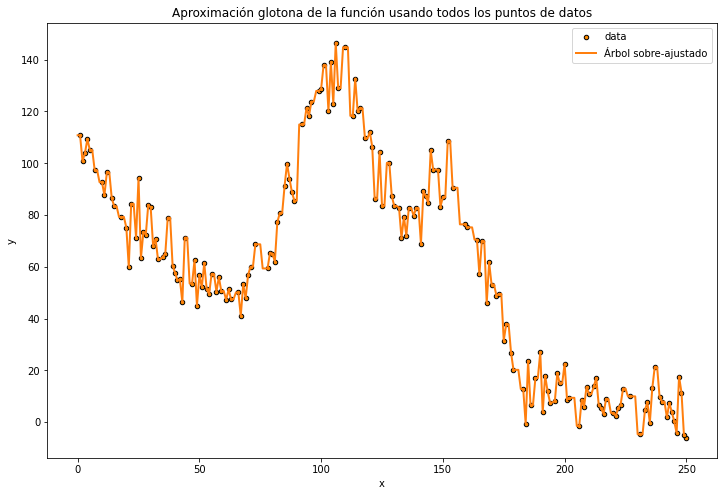
\includegraphics[height=6cm]{img/capN_sobreajuste_arbol.png}\\
	\caption{Aproximación de una función usando todos los puntos de entrenamiento (árbol sobreajustado).}
\end{figure}

Una manera más inteligente consiste en agrupar ciertos puntos y hacer una interpolación usando la media de estos. El desafío es encontrar una partición conveniente del dominio de los datos de modo que al predecir un punto de nuestra función, tomar la media de los datos de entrenamiento para el subconjunto correspondiente resulte en una buena aproximación.

\begin{figure}[h]
	\centering
	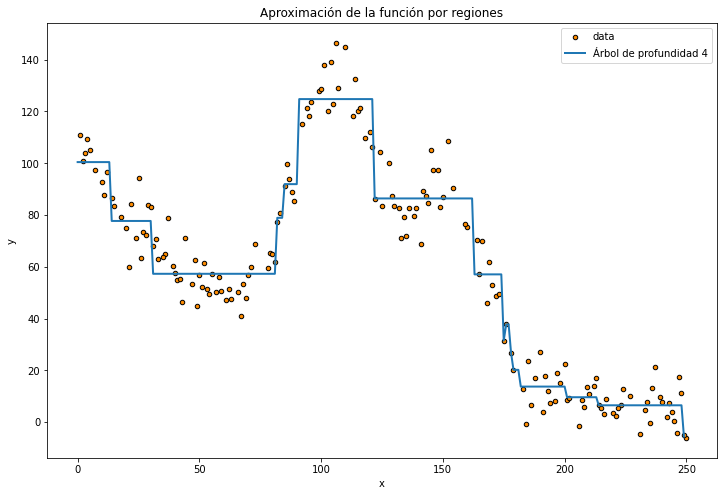
\includegraphics[height=6cm]{img/capN_buen_arbol.png}\\
	\caption{Aproximación de una función con un árbol de profundidad adecuada.}
\end{figure}


\subsubsection{Algoritmo \textit{CART}}

Los árboles (de regresión) corresponden a ejecutar lo anterior de manera recursiva. Primero, necesitamos una algún criterio que nos indique si realizar un corte vale o no la pena. Para esto podemos definir el costo para un conjunto $D$ de datos como sigue:

\begin{equation}
    cost(D) = \sum_{i \in D} (y_i - \bar y)^2 \,,
\end{equation}

con $\bar y = \frac{1}{|D|} \sum_{i \in D} y_i $. Notemos como este costo es proporcional a la varianza empírica del conjunto D, con lo cual pedir bajo costo en los grupos de una partición se traduce en pedir que los datos estén cercanos a la media de tal subconjunto. Con esto podemos armar un algoritmo de base recursivo que genere un árbol de regresión.


\begin{algorithm}[H]
  \caption{Ajuste de árboles (CART)
    \label{alg:CART}}
  \begin{algorithmic}[1]
    \Function{ajusteArbol}{$nodo, D, profundidad$}
      \State $j^*, t^* = \arg\min_{j \in \{1,\dots,m\}, t \in \Gamma_j} \left[ cost(D_L(j,t)) + cost(D_R(j,t)) \right]$

        $D_L(j,t) = \{(x^{(i)}, y^{(i)}) : x_j^{(i)} \leq t \}$, $D_R(j,t) = \{(x^{(i)}, y^{(i)}) : x_j^{(i)} < t \}$
      
      \If{criterio\_de\_parada($costo, profundidad, D_I, D_D$)}:
        \Return{nodo}
      \Else
        \State $nodo$.izquierda = ajusteArbol($nodo, D_I, profundidad + 1$)
        \State $nodo$.derecha = ajusteArbol($nodo, D_R, profundidad + 1$)
        
        \Return{nodo}
      \EndIf
    \EndFunction
  \end{algorithmic}
\end{algorithm}

Nótese que esto no necesariamente encontrará el árbol binario óptimo. Se prefiere este método voraz pues ajustar un árbol binario óptimo es un problema NP completo. En particular notemos como vamos separando coordenada por coordenada, lo cual nos hace ganar en interpretabilidad. Por otro lado, el 
 criterio de parada lo discutiremos más adelante.

Siguiendo el algoritmo anterior obtendremos una partición. Podemos enumerar los nodos de 1 hasta K, con lo cual recuperamos la forma de base adaptativa:

\begin{equation}
    f(x) = \mathbb{E}[y | x] = \sum^K_{k=1} w_k \phi_k(x) \,,
\end{equation}

con $\phi_k(x) = \mathbf{1}_{D_k}(x)$ y $w_k = \frac{1}{|D_k|} \sum_{x^{(i) \in D_k}} y^{(i)}$. Como se señaló en la intuición, escogeremos la media de los datos en el subconjunto como predicción. Esto se justifica pues aquel valor es el que minimiza el error cuadrático. Podríamos también aprender un modelo simple (por ejemplo un regresor de mínimos cuadrados) de manera local en cada partición, sin embargo como hemos escogido la partición de manera que minimice la varianza, es razonable pensar que la media será una aproximación suficientemente buena.


\subsubsection{Criterios de corte para clasificación}

En el algoritmo CART hicimos uso de la función costo, que nos mostraba cuánto variaban los miembros de un intervalo respecto de la media. Podemos generalizar este mismo principio para clasificación, donde intentaremos caracterizar la impureza de etiquetas para un conjunto de manera adecuada. Primero tomemos el vector de probabilidades de pertenencia a una clase, condicionado a estar en un nodo. Sea $\mathcal{C}$ el conjunto de clases,

\begin{equation}
    \hat \pi_c (D) = \frac{1}{|D|} \sum_{x^{(i) \in D}} \mathbf{1}_{y=c}(y^{(i)}) \hspace{1cm} \,, \forall c \in \mathcal{C} \,.
\end{equation}

Usando esto, predecir la probabilidad de que un punto pertenezca a cada clase estará dado por el vector de fracciones empírica $\hat \pi$ correspondiente al nodo al cual pertenezca el dato en cuestión. Usemos este mismo vector para definir los criterios de impureza por nodo (ignoraremos la dependencia de D en el vector de probabilidades para simplificar la notación) \cite{breiman_1984}.

\begin{itemize}
    \item \textbf{Tasa de error} \\
    Sea $\hat y = \arg\max_{c \in \mathcal{C}} \hat \pi_c$ la clase más probable. El error estará dado por
    \begin{equation}
        cost(D) = \frac{1}{|D|} \sum_{x^{(i) \in D}} \mathbf{1}_{y = \hat \y}(y^{(i)}) = 1 - \hat \pi_{\hat y}
    \end{equation}
    El problema de este criterio es su poca sensibilidad a cambios en el vector de probabilidad. Los siguientes dos criterios mejoran esta situación.

    \item \textbf{Gini} \\
    Corresponde a la tasa de error esperado:
    \begin{equation}
        cost(D) = \sum_{c \in \mathcal{C}} \hat \pi_c (1 - \hat \pi_c) = 1 - \sum_{c \in \mathcal{C}} \hat \pi_c^2
    \end{equation}

    \item \textbf{Entropía} \\
    También llamada log-pérdida y muchas veces denotada por $H(\hat \pi)$, esta métrica está dada por:
    \begin{equation}
        cost(D) = - \sum_{c \in \mathcal{C}} \hat \pi_c log(\hat \pi_c) \,.
    \end{equation}
    Esta elección de perdida tiene justificación en la Teoría de la Información. En particular, su uso como criterio de corte equivale a la minimización de la entropía cruzada.
\end{itemize}

% En la figura se grafican los costos en función de la probabilidad de una clase en el caso clasificación binaria. 
Consideremos el ejemplo de clasificación binaria.  % TO DO: agregar imagen, descomentar linea anterior y borrar esta
Notemos que para las tres el máximo está cuando tenemos 50/50 de datos para cada clase en el nodo en cuestión, que es justamente el caso de mayor heterogeneidad de los datos. Por el contrario, los valores son cero cuando el conjunto tiene miembros de una sola clase. La sensibilidad antes mencionada se desprende de esto. En el caso de clases impuras, el error de clasificación está siempre por debajo de los otros criterios, que castigan más fuertemente la impureza.

% insertar figura


\subsubsection{Evitar sobreajuste: detención temprana y poda}

Una primera estrategia para evitar el sobreajuste del árbol es la \textbf{detención temprana}, i.e., evitar que se siga particionando el espacio. A continuación mencionaremos algunos de los varios criterios. Estos se aplican como un criterio a verificar antes de seguir partiendo nodos en el algoritmo \ref{alg:CART} (CART):

\begin{itemize}
    \item \underline{Máxima profundidad}:
    se puede imponer una profundidad máxima, de modo que una vez alcanzada esta no se separe más el nodo en cuestión.

    \item \underline{Número mínimo en nodo}: si un nodo contiene muy pocos datos entonces partirlo puede resultar en nodos con muy pocos datos (a este fenómeno se le llama fragmentación de datos). Podemos considerar o bien un entero o bien un porcentaje mínimo de los datos totales.

    \item \underline{Mínima reducción de costos}: Dados lados izquierdos y derechos de un corte, consideremos la reducción en costo como:
    \begin{equation}
        \Delta = cost(D) - \left[ \frac{|D_L|}{|D|} cost(D_L) + \frac{|D_R|}{|D|} cost(D_R) \right]
    \end{equation}
    Esta métrica de reducción de costos normalizada nos permite definir un criterio de parada donde no cortaremos el nodo si los nodos resultantes no inducen una reducción significativa. 
\end{itemize}

Los criterios anteriores inducen hiperparámetros que pueden ser
escogidos en una búsqueda de grilla.

La \textbf{poda} es otra estrategia para evitar el sobreajuste y disminuir la complejidad del árbol. Esta consiste en ajustar un árbol uno (posiblemente con criterios de parada anteriormente expuestos) y luego podarlo, que corresponde a elegir un sub-árbol (i.e., “podar” nodos). El conjunto de todos los subárboles de un árbol de decisión es potencialmente muy elevado. Es por esto que se elegirá un conjunto adecuado de subárboles, de modo que sea razonable comparar su rendimiento para elegir la mejor opción.

Primero consideraremos una métrica $R(T)$ que nos de una noción de costo para un árbol $T$. Típicamente se usará la suma de las tasas de errores (definidas anteriormente para clasificación y regresión) sumadas para cada hoja. Consideremos que el tamaño de un árbol $T$ es su número de hojas y denotemos aquello por $|T|$. Lo anterior nos permite definir una métrica que incorpora tanto el error como el tamaño de un árbol:

\begin{equation}
    R_\alpha (T) = R(T) + \alpha |T|
\end{equation}

Esta expresión se puede interpretar como agregar una penalización por complejidad si pensamos $\alpha$ como costo en complejidad de un nodo terminal. Notemos que a medida que se aumenta $\alpha$ más estaremos prefiriendo un árbol con menos hojas, por ende la métrica es sensible a tal hiperparámetro. Usaremos este hecho para construir un algoritmo que seleccione árboles adecuados de los cuales seleccionar el mejor, donde la idea se resume a continuación:

Dado el árbol original $T_0$, el objetivo será construir una sucesión de árboles $T_0, T_1, \dots, T_m$, disminuyendo en cada paso el número de nodos terminales y donde $T_m$ es simplemente el nodo raíz. Para aquello notemos que pese a que el número de subárboles de $T_0$ es potencialmente grande, siempre es un número finito. Con esto, si $T(\alpha)$ es el árbol que minimiza el costo $R_\alpha$, entonces al aumentar $\alpha$, aquel árbol seguirá siendo el óptimo hasta llegar a un punto de salto $\alpha'$, en el cual un nuevo árbol $T(\alpha')$ se convierte en el mínimo y así sucesivamente.

Este punto se encuentra guardando los costos y tamaños de subárboles dados por podar en algún nodo. Cuando podemos esto consistirá en deshacer la separación hecha en el nodo en cuestión, con lo cual nos quedará la estimación que teníamos para el subconjunto original sin separar partes derecha e izquierda. La idea es encontrar iterativamente el nodo más débil que podamos podar.

A continuación el algoritmo de poda \cite{ripley}, luego del cual podemos enunciar los resultados que lo justifican. Precisemos que $T_t$ se refiere al subárbol cuya raíz (nodo del cual salen todas las ramas) es el nodo $t$.

\begin{algorithm}[H]
  \caption{Poda de costo-complejidad
    \label{alg:poda}}
  \begin{algorithmic}[1]
    \Function{sucesionArboles}{$T$}
    \State\textbf{set} $k=0$, $T_0= T$, $\alpha = \infty$
    \For{$t$ \textbf{in} {nodos no terminales desde abajo hacia arriba}}:
        \State calcular $R(T_t)$ y $|T_t|$ sumando sobre los descendientes e incluyendo contribuciones en $t$
        \State \textbf{set} $g(t) = \frac{R(t) - R(T_t)}{|T_t| - |t|}$
        \State \textbf{set} $\alpha = \min(\alpha, g(t))$
    \EndFor
    \For{$t$ \textbf{in} {nodos no terminales de arriba hacia abajo}}:
        \If{$g(t) = \alpha$}
            \State Reemplazar $T_t$ por $t$ (podar)
                \State \textbf{set} $k = k+1$, $\alpha_k = \alpha$ y $T_k = T$
                \If{$T$ es un árbol de un sólo nodo}
                    \State\Return{$\alpha_1, \dots, \alpha_m$, $T_1, \dots, T_m$}
                \Else
                    \State Ir a paso (3)
                \EndIf
        \EndIf
    \EndFor
    \EndFunction
  \end{algorithmic}
\end{algorithm}

Notemos que la función $g$ nace de querer despejar aquel $\alpha$ que le de suficiente peso al tamaño del árbol de modo que $R_\alpha (T_t) = R_\alpha(t)$, esto es

\begin{equation}
    R(T_t) + \alpha |T_t| = R(t) + \alpha |t| \Longleftrightarrow  \alpha = \frac{R(t) - R(T_t)}{|T_t| - |t|} \,.
\end{equation}

\begin{lemma}[Consistencia de poda costo-complejidad]

    Sea $g(t,T) = \frac{R(t) - R(T_t)}{|T_t| - |t|}$ para un nodo $t$ y un subárbol $T_t$ con raíz en $t$.
    \begin{enumerate}
        \item El resultado de podar en un nodo $t$ si $R_\alpha(t) \leq R_\alpha(T_t)$ al visitar los nodos de abajo hacia arriba, el árbol resultante es
        \begin{equation}
            T(\alpha) = \arg\min_{\tilde T \leq T} R_\alpha(\tilde T)
        \end{equation}

        \item Sea $\tilde \alpha = \min \{ g(t,T) :t \text{ es nodo no terminal de } T \} $, podar en todos aquellos nodos que cumplan $g(t,T) = \tilde \alpha$ resulta en $T(\tilde \alpha)$. Además, $g(t, T(\tilde \alpha)) > \tilde \alpha$ para todo nodo $t$ no terminal en $T(\tilde \alpha)$.

        \item Para $\beta > \alpha$, $T(\beta)$ es subárbol de $T(\alpha)$ y es el resultado de $\beta$-podar $T(\alpha)$.
    \end{enumerate}
\end{lemma}

Hasta ahora lo único que hemos hecho es definir una secuencia de árboles conveniente, sin embargo esto nos deja la responsabilidad de elegir un buen árbol para nuestro estimador final. Lo que tenemos hasta ahora son:

\begin{equation}
    T = T_0 < T_1, \dots, T_{m-1} < T_m \,,
\end{equation}

donde $<$ denota la relación ``ser subárbol''. Además tenemos una sucesión $\alpha_0 < \alpha_1 < \dots < \alpha_m$ (donde en este caso $<$ es la relación ``menor a'' usual en los números reales). Es de esperar que el error de entrenamiento aumente a medida que aumentamos $\alpha$ . Este no es necesariamente el caso en un conjunto de testeo, pues es probable que los árboles con muchas hojas sean resultado de un sobreajuste. Una manera razonable de escoger un árbol final es tomar aquel que tenga menos error en un conjunto de entrenamiento o validación. También podemos hacer uso de técnicas como validación cruzada.


\subsubsection{Interpretabilidad}

Nos hemos restringido al ajuste de un árbol, sin embargo es útil pensar en las ventajas que puede tener este tipo de modelos respecto a otros vistos en el curso. Por su naturaleza, los árboles tienen una buena capacidad de interpretabilidad. % Para graficar esto tomemos un ejemplo.

Usando las variables que se usaron para cortar cada nodo y los valores para el corte óptimo, podemos explicar la diferencia en estimaciones obtenidas. A esto lo llamamos capacidad de interpretación, y es importante a la hora de usar aprendizaje de máquinas para decisiones con repercusión en el mundo real.

En este caso se ha ajustado un árbol para clasificar imágenes de dígitos escritos a mano (dataset \textit{mnist}). Acá, cada variable corresponde a un pixel en particular, que en La Figura \ref{fig:arbol_interpretabilidad} están destacados en rojo. Cuando se llegan a hojas del árbol se logra, en muchos casos, distinguir dígitos. Por otro lado, nodos intermedios denotan conjuntos impuros (con varios dígitos posibles), de los cuales es necesario realizar un corte. Se vislumbran entonces que pixeles son más importantes a la hora de distinguir dígitos y que desencadenan en la decisión tomada por el árbol de clasificación.

\begin{figure}[H]
    \centering
    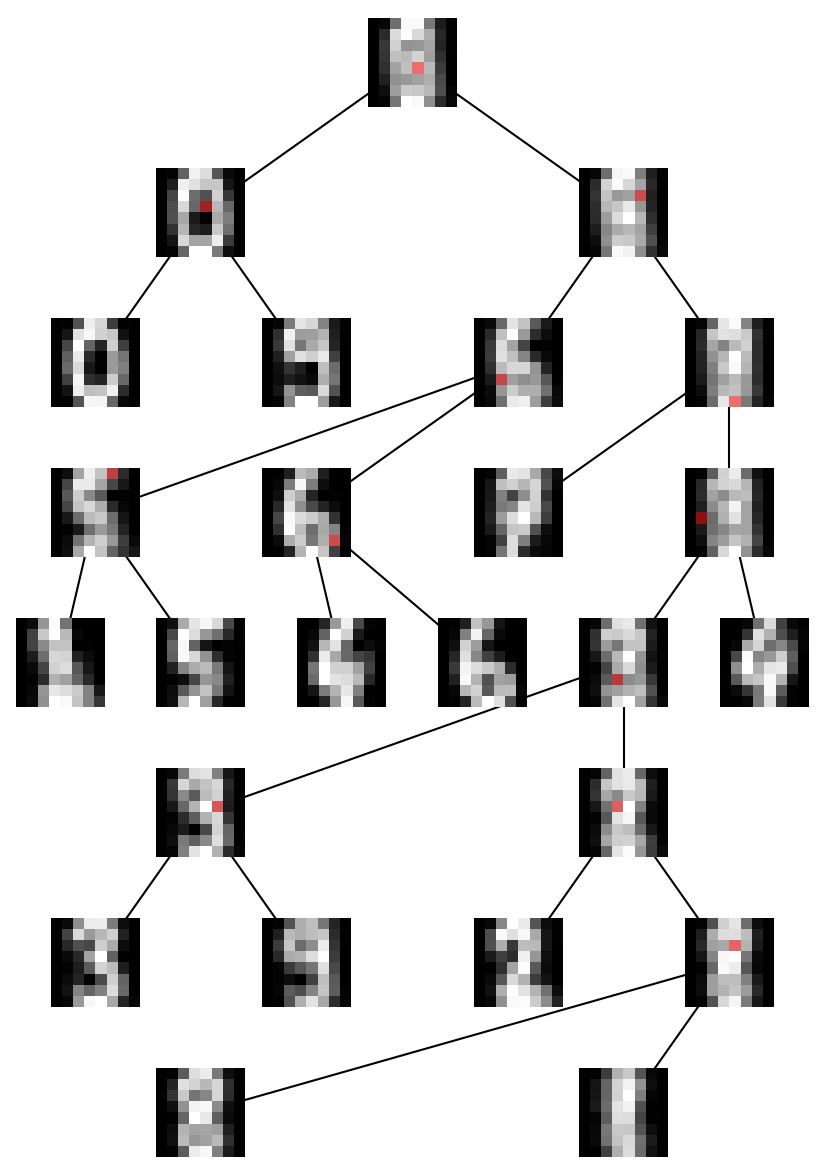
\includegraphics[width=0.57\textwidth]{img/capN_interpretacion_arbol.png}\\
    \caption{Visualización de un árbol de clasificación para el dataset \textit{mnist}.}
    \label{fig:arbol_interpretabilidad}
\end{figure}


\subsection{Bagging}
\label{sec:bagging}

Esta sección tiene como objetivo mostrar un método para ensamblar modelos generales \cite{bagging}. Antes de discutirlo, necesitamos la noción del concepto \textit{bootstrapping}.

\subsubsection{Método Bootstrapping}

En palabras simples, \textit{bootstrapping} es un procedimiento que consiste en escoger aleatoriamente puntos de datos con repetición, desde el conjunto de datos original. La repetición de esto nos permite acceder a varias distribuciones que intentan aproximar la original.

\begin{figure}[h]
	\centering
	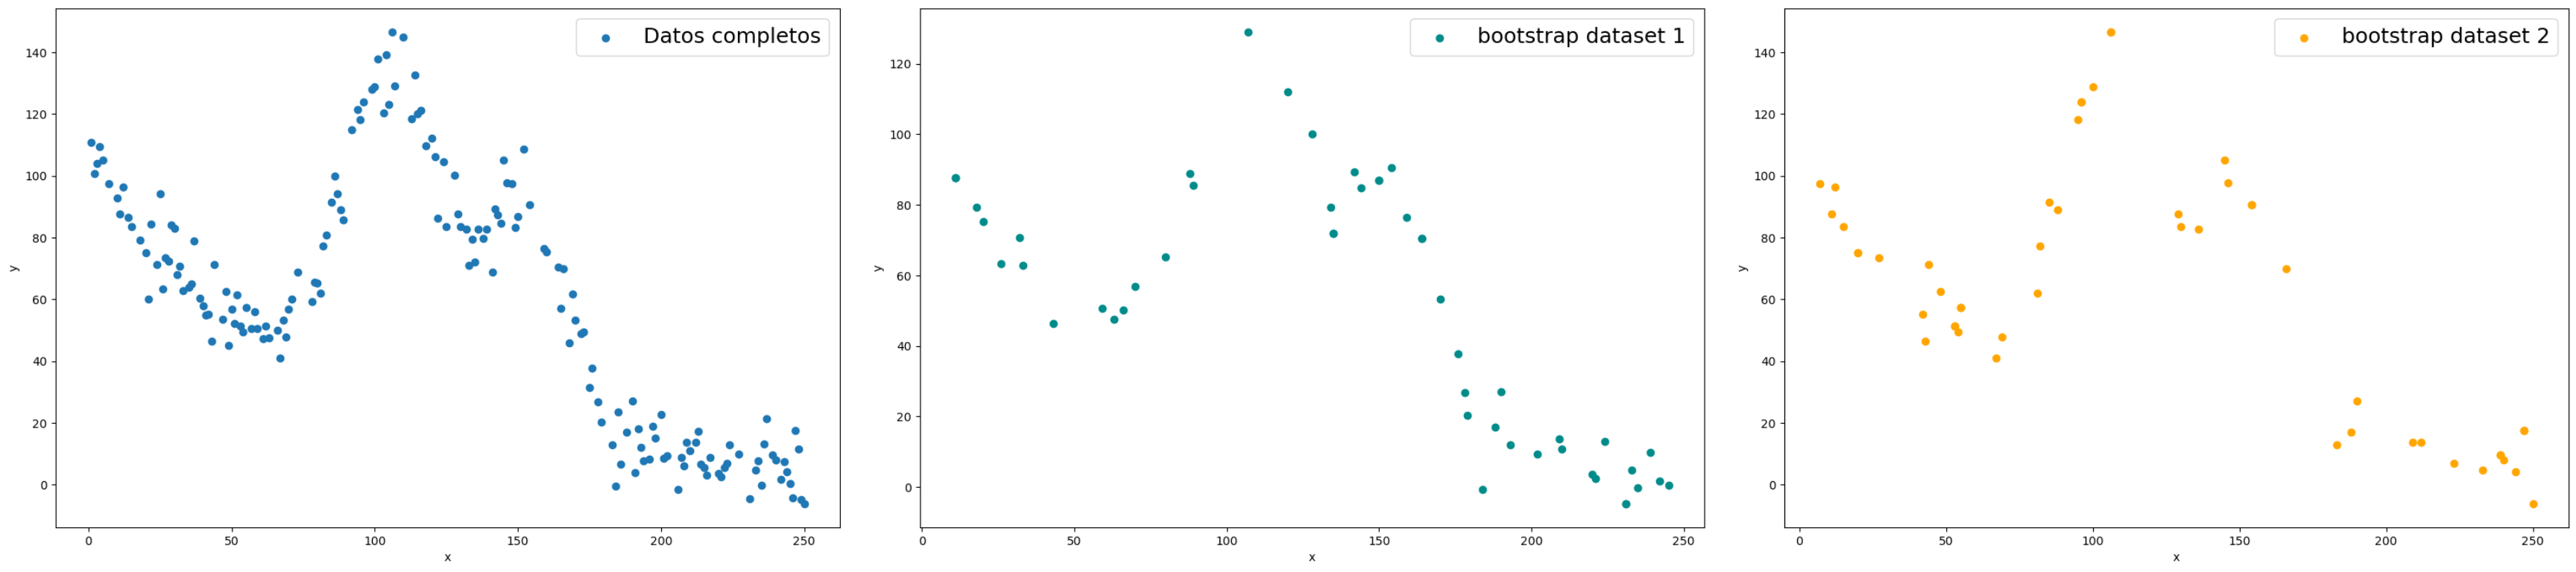
\includegraphics[width=0.9\textwidth]{img/capN_bootstrapping.png}\\
	\caption{Ejemplo de conjuntos de datos muestreados con \textit{bootstrapping}.}
\end{figure}

Con estas distribuciones, que serán típicamente de menor tamaño, se espera capturar la variabilidad de los datos. Un ejemplo de uso es ajustar modelos a las diferentes distribuciones de \textit{bootstrap}. Una idealización de lo anterior se muestra en La Figura \ref{fig:bagging}, donde se usan dos re-muestreos (con repetición) para el ajuste.

\begin{figure}[H]
    \centering
    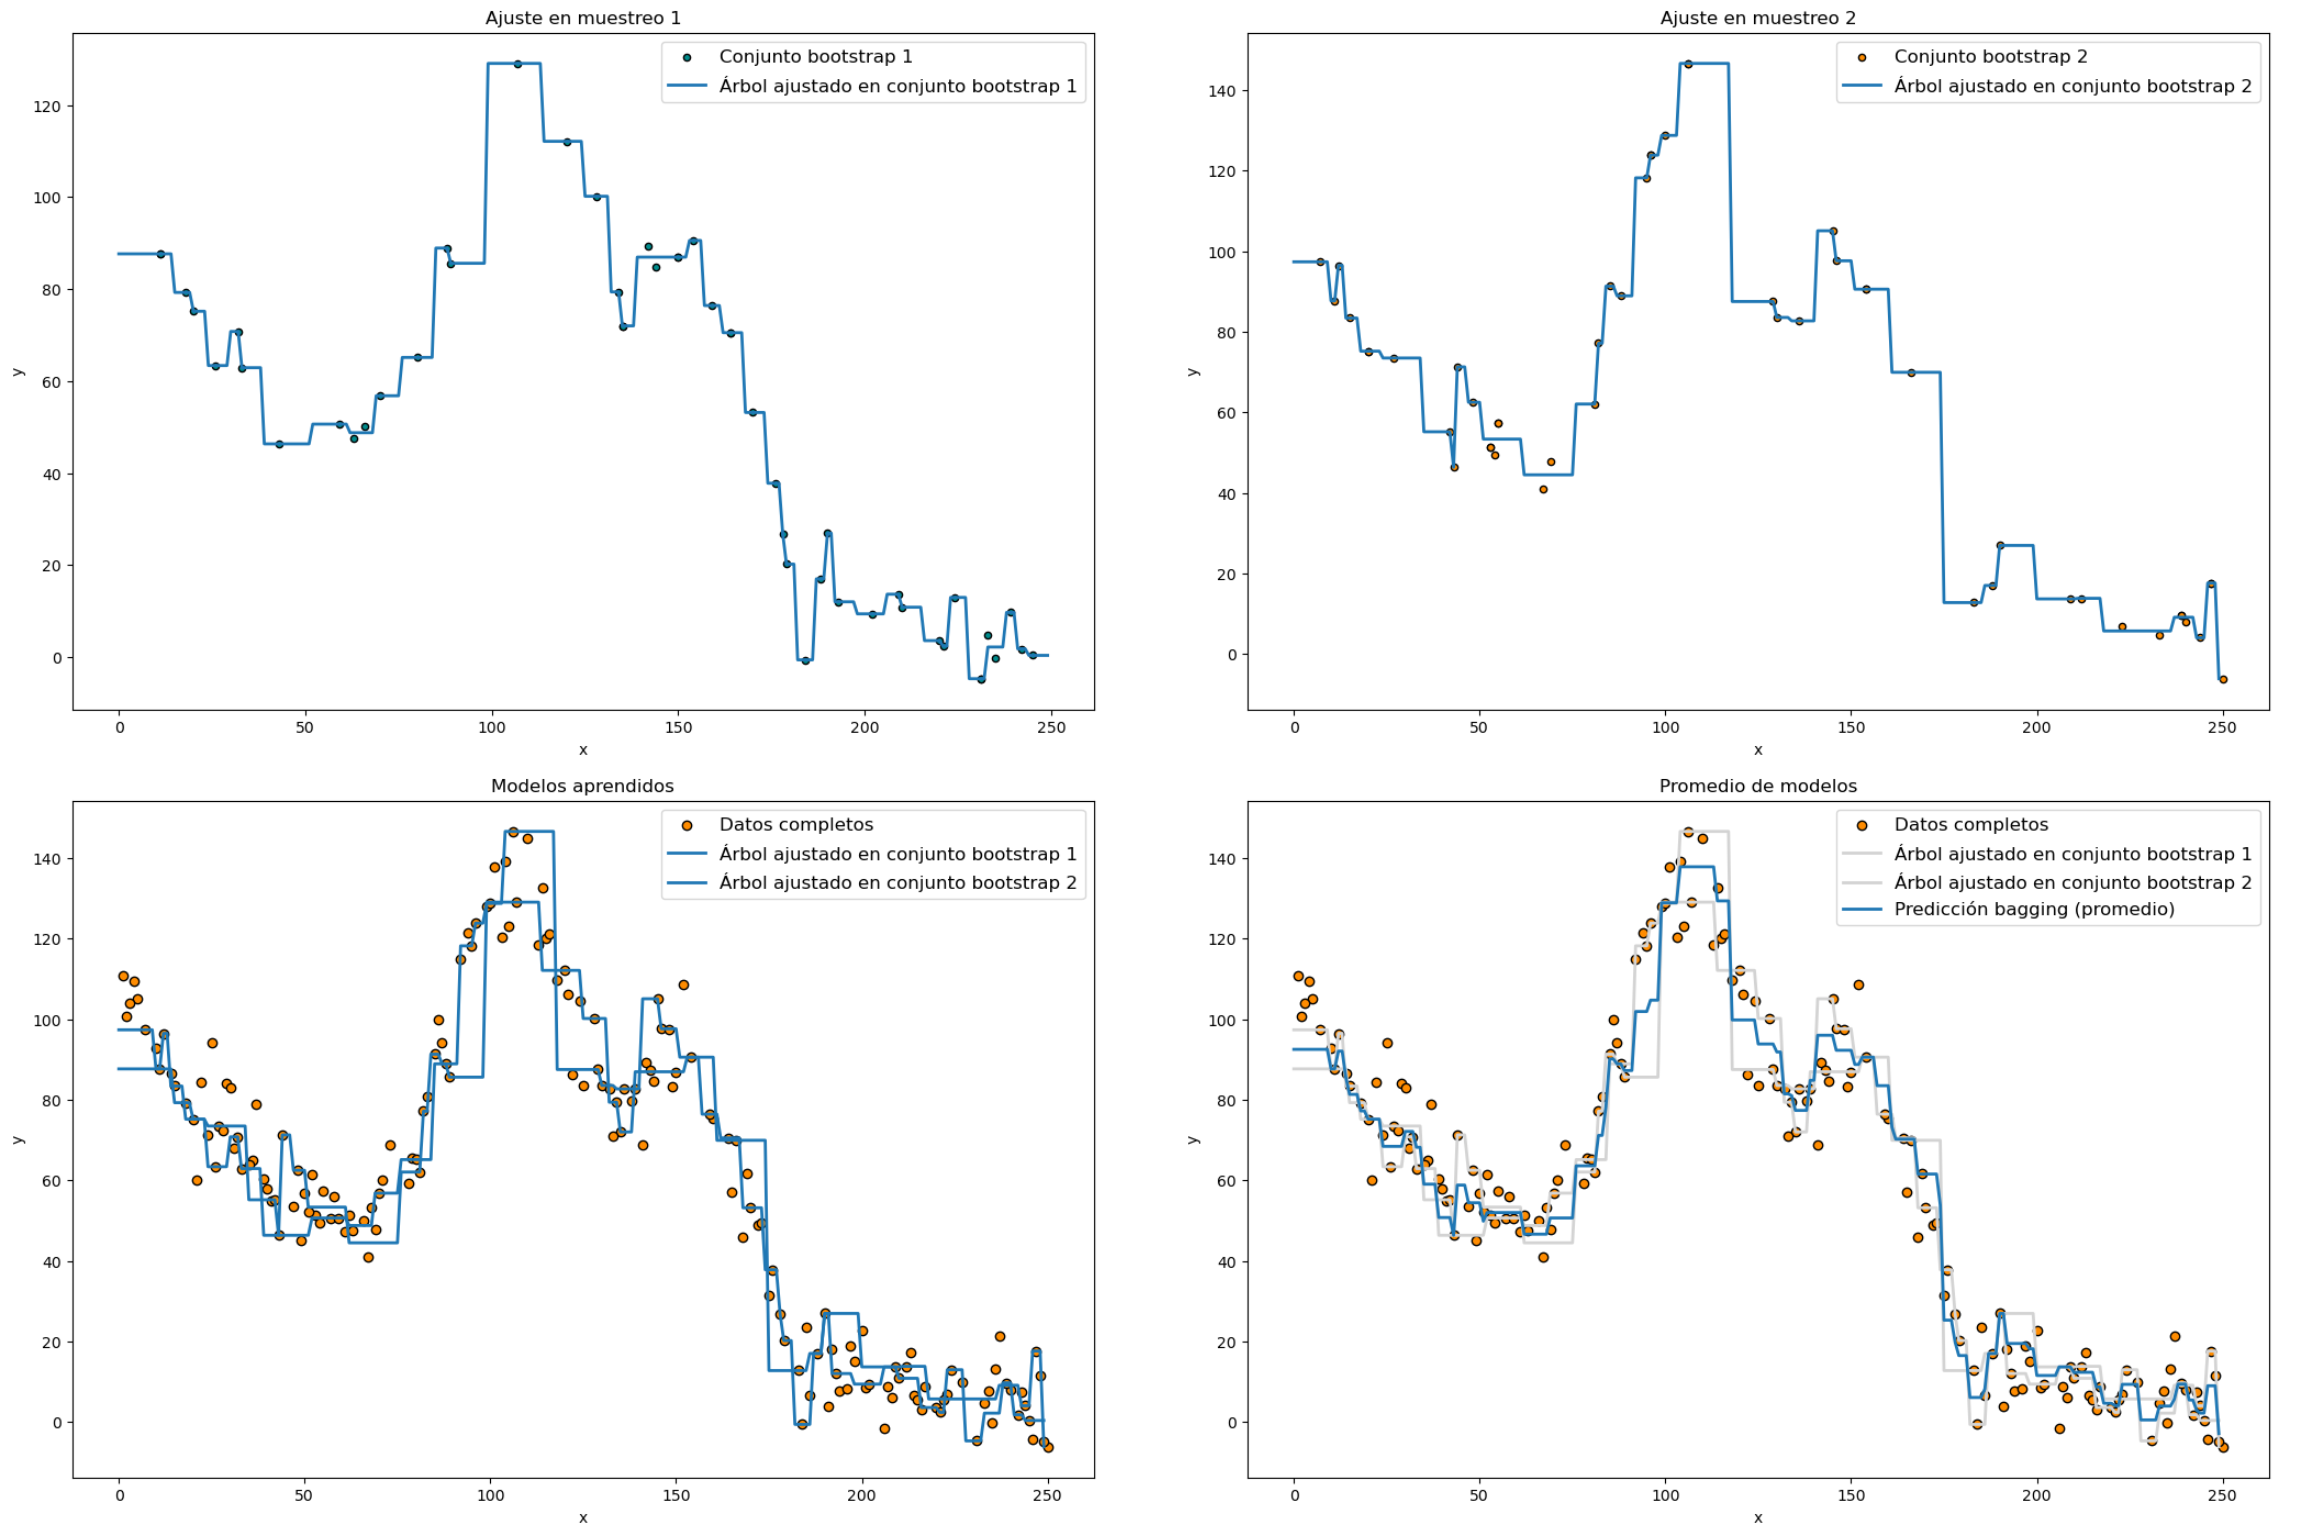
\includegraphics[width=0.95\textwidth]{img/capN_bagging_ejemplo.png}\\
    \caption{Ejemplo de predicción \textit{bagging} (promedio) usando dos modelos de árboles.}
    \label{fig:bagging}
\end{figure}

Podemos luego ver la diferencia de los estimadores versus los datos originales. Hacer esto varias veces nos puede dar una noción punto por punto de la varianza en ciertos puntos del input. Es interesante notar que si en vez de samplear desde los datos originales considerásemos un modelo con ruido Gaussiano y muestreamos de esa distribución obtendríamos el equivalente modelo ajustado con mínimos cuadrados a medida que consideramos más distribuciones.

El caso general es consistente con encontrar un modelo que maximice la verosimilitud. Usaremos este principio para definir \textit{Bagging}, que será usar la información de varios modelos aprendidos en distintas distribuciones de \textit{bootstrap}.


\subsubsection{Bagging: agregación de modelos}

Sea $\{\mathcal{D}^{(b)}\}^B_{b=1}$ una colección finita de conjuntos de datos tomados con el método \textit{bootstrap}, es decir, muestreando repetidamente del conjunto de datos original $ \mathcal{D} = \{(x_n,y_n)\}^N_{n=1}$ con repetición. Supongamos que en cada conjunto ajustamos un modelo, con lo cual tenemos $B$ modelos: $\{ \varphi(x,\mathcal{D}^{(b)}) \}^B_{b=1}$.

El estimador resultante de usar el método \textit{bagging} en cada caso estará dado por:

\begin{equation}
    \varphi_{bagging}(x) = \frac{1}{B} \sum^B_{b=1} \varphi(x,\mathcal{D}^{(b)}) \,.
\end{equation}

El nombre \textbf{\textit{bagging}} proviene de la combinación de \textit{\textbf{b}ootstrap} y \textit{\textbf{agg}regaga\textbf{ting}}, lo último correspondiendo a agregación de modelos, lo cual viene de usar el promedio. En el caso de clasificación, lo usual es votar, i.e., tomar la clase que sea preferida por la mayor cantidad de modelos.

Es natural preguntarse en qué casos será conveniente usar \textit{bagging} por sobre un modelo ajustado en el conjunto de datos original. La respuesta a esto dependerá de la sensibilidad de los modelos de base. En efecto denotemos 

\begin{equation}
    \varphi_{bagging}(x) = \mathbb{E}_{ \tilde D \sim D } \left[ \varphi(x,\tilde D) \right] \,,
\end{equation}

donde $\tilde D \sim D$ denota que el conjunto de datos usado para ajustar el modelo fue tomado usando muestreos que distribuyen de acuerdo a la distribución de probabilidad del modelo original. Usando esto, podemos acotar el error esperado usando que:

\begin{equation}
    \mathbb{E}_{ \tilde D \sim D } \left[ y - \varphi(x,\tilde D) \right]^2 = y^2 - 2 y \mathbb{E}_{ \tilde D \sim D } \left[\varphi(x,\tilde D) \right] + \mathbb{E}_{ \tilde D \sim D } \left[\varphi^2(x,\tilde D) \right] \,.
\end{equation}

Además, gracias a la desigualdad de Cauchy-Schwartz, podemos acotar el tercer término: 
\begin{equation}
\label{eq:bagging_CS}
    \mathbb{E}_{ \tilde D \sim D } \left[\varphi^2(x,\tilde D) \right] \geq \mathbb{E}_{ \tilde D \sim D } \left[\varphi(x,\tilde D) \right]^2 \,.
\end{equation}

Con esto queda:

\begin{align}
    \mathbb{E}_{ \tilde D \sim D } \left[ y - \varphi(x,\tilde D) \right]^2 & \geq (y - \mathbb{E}_{ \tilde D \sim D } \left[\varphi(x,\tilde D) \right] )^2
    \\ & = (y - \varphi_{bagging}(x))^2 \,.
\end{align}

Luego considerando todos los datos obtenemos que el error cuadrático promedio de los modelos será mayor al error cuadrático del estimador \textit{bagging}. El margen de mejora depende solamente de cuán fuerte es la desigualdad de la inecuación \ref{eq:bagging_CS}, que podemos re-escribir como

\begin{equation}
    Var_{ \tilde D \sim D } \left[\varphi(x,\tilde D) \right] = \mathbb{E}_{ \tilde D \sim D } \left[\varphi^2(x,\tilde D) \right] - \mathbb{E}_{ \tilde D \sim D } \left[\varphi(x,\tilde D) \right]^2 \geq 0 \,.
\end{equation}

Dicho de otro modo, la varianza del modelo para las distribuciones de \textit{bootstrap} serán esenciales para que existan ganancias significativas. El método \textit{bagging} es entonces recomendable para modelos \textbf{inestables}, i.e., que varíen más bruscamente con cambios en los datos. Para modelos que no varíen demasiado con las distintas distribuciones \textit{bagging} no introduce mejora (y en la práctica puede empeorar la predicción).


\subsubsection{Bosques aleatorios y variaciones}

En principio es razonable pensar que la técnica \textit{bagging} funcionará con árboles, pues estos son relativamente sensibles a los datos utilizados (sobretodo si no podamos o si no usamos criterios de parada exigentes). Justamente cuando tenemos árboles suficientemente profundos, podemos asumir que tendrán un sesgo muy pequeño. La técnica \textit{bagging} no afecta el sesgo de los estimadores, mejora sus resultados más bien reduciendo la varianza.

Supongamos que aprendemos $B$ árboles, cada uno en un conjunto de datos generados con \textit{bootstrapping}. Teóricamente cada estimador $\varphi(x,\mathcal{D}^{(b)})$ tendrá la misma varianza, que podemos denotar $\sigma^2$, pues los estimadores son independientes e idénticamente distribuidos. En la práctica los estimadores no son necesariamente independientes. Sea $\rho$ la correlación dos-a-dos de los estimadores. En este caso, la varianza del estimador \textit{bagging} (promedio) está dada por:

$$ \rho \sigma^2 + \frac{1 - \rho}{B} \sigma^2 \,, $$

a diferencia del caso i.i.d., para el cual la varianza final es

$$ \frac{1}{B}\sigma^2 \,. $$

En ambos casos la varianza se reduce al aumentar $B$, sin embargo el término $\rho \sigma^2$ nos restringe la reducción de varianza. La idea de los bosques aleatorios (conocidos como \textit{random forest} en inglés) será reducir la correlación de los estimadores para reducir la varianza sin afectar fuertemente el sesgo, y de esta forma reducir el error. Haremos esto seleccionando aleatoriamente variables con las cuales aprender cada árbol, como se señala en Algoritmo \ref{alg:RF} \cite{breiman2001random}.

\begin{algorithm}[H]
  \caption{Bosques Aleatorios
    \label{alg:RF}}
  \begin{algorithmic}[1]
  \Function{BosqueAleatorio}{$D, B$}
  \For{$b \in \{1,\dots,B\}$}
    \State Obtener $\mathcal{D}^{(b)}$ de $D$ con el método \textit{bootstrap}.
    \State Ajustar un árbol $T_b$ en $\mathcal{D}^{(b)}$ del modo siguiente:
        \For{nodo in $T_b$}
            \State seleccionar $m$ variables de las $p$ posibles
            \State seleccionar la mejor variable y corte
            \State partir del nodo según el corte
        \EndFor
    \EndFor
    \Return{$\{T_b\}^B_{b=1}$}
    \EndFunction
  \end{algorithmic}
\end{algorithm}

Para realizar las predicciones finales usamos:
$$ \varphi_{RF}(x) = \frac{1}{B} \sum^B_{b=1} T_b (x) \,, $$

o bien la clase con más votos en el caso de clasificación.

Lo aleatorio de los bosques aleatorios está en la selección de $m$ variables. El número $m$ es un parámetro en sí mismo, pero suele usarse $p/3$ para regresión y $\sqrt{p}$ para clasificación, donde $p$ es el número de parámetros.

Tanto en el caso de bosques aleatorios como en \textit{bagging} general, se dice que los estimadores no sobre-ajustan. Si bien esto es cierto en teoría, en la práctica es usual que muchas variables no sean útiles para la predicción. El efecto de la selección de variables hace que muchas veces se ignoren las pocas variables que si pueden explicar los datos. Es posible que muchos de los árboles tengan una expresividad innecesaria, al usar variables inútiles, y por ende resulten en una mala generalización.


\subsubsection{Árboles extremadamente aleatorios}

Una alternativa a los bosques aleatorios es usar un promedio de modelos pero aprendidos en el mismo conjunto de datos (i.e., sin el método bootstrap). La ``extrema'' aleatoriedad proviene de modificar el ajuste de arboles del siguiente modo:
\begin{itemize}
    \item Usar un subconjunto aleatorio de variables (como en bosques aleatorios).
    \item Para cada variable del subconjunto generar cortes de modo aleatorio, en vez de seleccionar el mejor de todos. De aquellos cortes generados, se escoge el mejor de acuerdo al criterio empleado.
\end{itemize}
A este método se le denomina árboles extremadamente aleatorios (\textit{ExtraTrees} en inglés). Aparte de la decorrelación de los estimadores, \textit{ExtraTrees} tiene una mejor eficiencia computacional que los árboles clásicos \cite{geurts2006extremely}.


\subsection{Boosting}
\label{sec:boosting}

En las sección \textit{bagging} aprendimos como mejorar conjuntamente una colección de estimadores, ajustados cada uno por separado. En tal configuración asumimos que los modelos son insesgados y nos enfocamos en reducir varianza. En esta sub-sección veremos el método \textit{boosting}, que ajusta un conjunto de modelos sesgados de manera adaptativa para reducir el sesgo del estimador final.

\subsubsection{Motivación: algoritmos fuertes versus débiles}

Antes de adentrar en detalles, recordemos las preguntas teóricas cuyas respuestas decantaron en el método final. En el análisis matemático de modelos predictivos es usual trabajar en el marco conceptual PAC, que significa \textbf{p}robablemente \textbf{a}proximadamente \textbf{c}orrecto. En tal contexto, solemos seleccionar estimadores que con alta probabilidad tengan un bajo error de generalización (que sean aproximadamente correctos). En términos matemáticos, solemos tomar $\epsilon > 0$, $0 < \delta < 1$ de modo que nuestro algoritmo se dirá PAC-aprendible si logra tener un error de a lo más $\epsilon$ con probabilidad $1-\delta$ \cite{schapire2012boosting}.

Por otro lado, podemos considerar un paradigma alternativo en el cual dado $\gamma > 0$ exijamos un modelo que tenga un error $\frac{1}{2} - \gamma$ con probabilidad menor a $\delta$. Dicho de otro modo, en vez de pedir una alta probabilidad de precisión arbitraria, pedimos que la probabilidad de que nuestro algoritmo sea peor que 50\% sea baja. A un algoritmo que cumpla esto se le llamará débilmente PAC-aprendible (en contraste con PAC-aprendible, que también se le denomina fuertemente PAC-aprendible en este contexto).

La intuición nos dice que como la débil PAC-aprendibilidad es menos ``exigente'' que la fuerte, habrán más algoritmos débiles que algoritmos fuertes. Esto resulta ser falso. \textit{boosting} en su sentido original es un algoritmo que al tomar un algoritmo débil es capaz de convertirlo en uno fuerte (en el sentido de PAC aprendibilidad). La existencia de algoritmos de \textit{boosting} implica la equivalencia de la débil y fuerte PAC-aprendibilidad.


\subsubsection{Algoritmo \textit{AdaBoost}}

Consideremos el caso en el que tenemos acceso a clasificadores de base que son débiles, en el sentido de ser ligeramente mejores que una elección por azar. Esta ligera mejora respecto de un modelo trivial es la única exigencia que se le da a los clasificadores de base. Estos serán tratados como caja negra y serán llamados como sub-rutina para mejorar la predicción final.

La clave del éxito para los métodos boosting es escoger los conjuntos de entrenamientos para los estimadores de base de tal modo que estos sean ``forzados'' a inferir nueva información de los datos que no estaba presente anteriormente. Al escoger puntos de datos en los cuales el rendimiento de los algoritmos de base son incluso peores que su rendimiento débil usual, podemos ajustar modelos débiles en ellos para acercarnos al rendimiento fuerte deseado. Esto se ilustra en La Figura \ref{fig:idea_boosting}.

\begin{figure}[h]
    \centering
    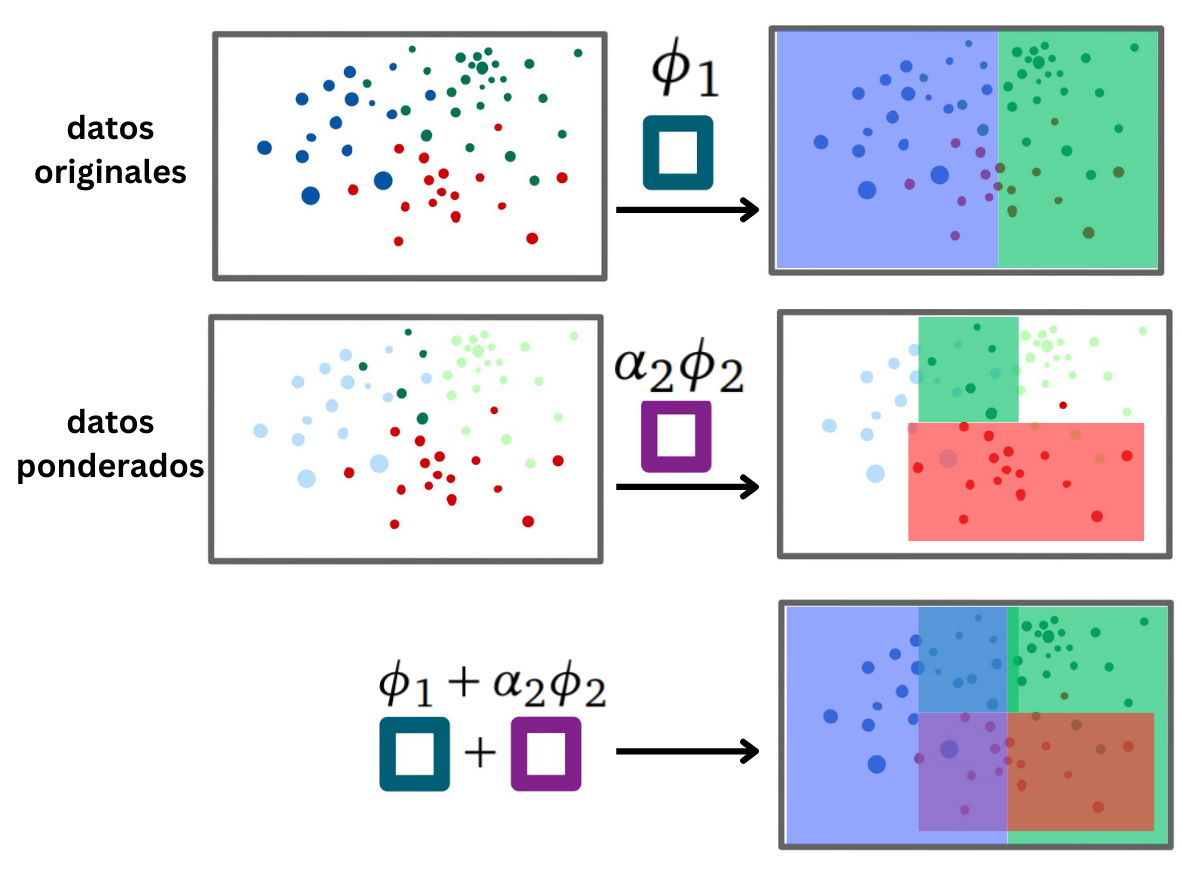
\includegraphics[width=0.8\textwidth]{img/CapN_idea_boosting.png}\\
    \caption{Intuición del método \textit{boosting}.}
    \label{fig:idea_boosting}
\end{figure}

Supongamos que tenemos un conjunto de datos $D = \{(x_i,y_i)\}^N_{i=1}$, donde N será el tamaño del dataset. Consideraremos únicamente el caso de clasificación binaria donde las etiquetas están dadas por el conjunto {-1,1}. Supongamos que tenemos un modelo $\phi_m$ que consideramos débil. Usando la heurística anterior, queremos ajustar un nuevo modelo débil $\phi_{m+1}$.

Usaremos la pérdida exponencial: $L(\phi) = e^{-y_i \phi(x_i)}$. Buscaremos minimizar esa pérdida, usando el estimador:
$$ \phi(x) = \phi_m(x) + \alpha_{m+1}\phi_{m+1}(x)\,, $$

con lo cual, debemos resolver

\begin{align}
    \min_{\alpha_{m+1}} L(\phi(x)) & = \min_{\alpha_{m+1}} \sum^N_{i=1} e^{-y_i (\phi_m(x_i) + \alpha_{m+1} \phi_{m+1}(x))} \\
    & = \min_{\alpha_{m+1}} \sum^N_{i=1} w_i^{(m)} e^{\alpha_{m+1} \phi_{m+1}(x)} \,,
\end{align}

donde definimos $w_i^{(m)} = e^{-y_i \phi_m(x_i)}$ para $i = 1,\dots,N$, que lo podemos interpretar como el dataset original ponderado por el error (exponencial) del modelo $\phi_m$.

\begin{lemma}
    El $\alpha_{m+1}$ que minimiza la función anterior está dado por
    \begin{equation}
        \alpha_{m+1} = \frac{1}{2} \log(\frac{1-\epsilon_m}{\epsilon_m})\,,
    \end{equation}
    donde  $\epsilon_m = \displaystyle \frac{ \sum_{y_i \neq \phi_m(x_i)} w_i}{\sum_{i=1}^N w_i} $.
\end{lemma}

El desarrollo anterior resulta en el algoritmo \ref{alg:AdaBoost} \cite{freund1997decision,ESLbook}. Se demostró que puede convertir clasificadores débiles en un clasificador débil (para el caso binario).

\begin{algorithm}[H]
  \caption{AdaBoost
    \label{alg:AdaBoost}}
  \begin{algorithmic}[1]
  \Function{AdaBoost}{$D, M$}
  \State Set $w_i = \frac{1}{N}\,\forall i=1,\dots,N$ (con $N$ tamaño del dataset)
    \For{$m = 1, \dots, M$}
        \State Entrenar un modelo débil $\phi_m$  minimizando $\displaystyle \sum_{y_i \neq \phi_m(x_i)} w_i$
        \State Set $\epsilon_m = \displaystyle \frac{ \sum_{y_i \neq \phi_m(x_i)} w_i}{\sum_{i=1}^N w_i}$
        \State Set $\alpha_{m} = \frac{1}{2} log(\frac{1 - \epsilon_m}{\epsilon_m})$
        \State Set $w_i = w_i \cdot \exp(-y_i \phi_m(x_i) \alpha_m)$ % si $y_i \neq \phi_m(x_i)$ (opcional)
        \State Actualizar $\{w_i\}^N_{i=1}$ de modo que $\sum^N_{i=1} w_i = 1$
    \EndFor
    \Return{$\phi(x) = signo \left(\sum^M_{m=1} \alpha_m \phi_m(x)\right)$}
    \EndFunction
  \end{algorithmic}
\end{algorithm}

Recordando las nociones de débil y fuerte aprendibilidad, podemos enunciar el siguiente resultado:

\begin{theorem}[Boosting]
    Una clase objetivo $\mathcal{C}$ es (eficientemente) debilmente aprendible, si y solo si es (eficientemente) fuertemente aprendible
\end{theorem}

Es evidente que un modelo fuerte es en particular débil. Por el contrario, la conversa (débil PAC-aprendibilidad implica fuerte PAC-aprendibilidad) es resultado de aplicar el algoritmo AdaBoost a modelos de base débiles como caja negra. Esta equivalencia fue presentada por Yoav Freund y Robert Schapire, quienes ganaron el prestigioso premio Gödel gracias a esta contribución.

Si bien la demostración del teorema tiene elementos que escapan el enfoque de este curso, enunciamos a continuación un resultado que nos da una idea de la capacidad de AdaBoost para reducir el error (en el conjunto de entrenamiento) a medida que aumentamos la cantidad de estimadores.

\begin{theorem}
    Sea $\gamma_m = \frac{1}{2} - \epsilon_m$ y sea $D_1$ una distribución inicial arbitraria sobre el dataset de entrenamiento. El error de entrenamiento (ponderado por los pesos) del clasificador combinado con respecto a $D_1$ está acotado por:
    \begin{equation}
        \mathbb{P}_{i \sim \mathcal{D}_1}(\phi(x_i) \neq y_i) \leq \prod^M_{m=1} \sqrt{1-4\gamma^2_m} \leq e^{-2\sum^M_{m=1} \gamma^2_m} \,.
    \end{equation}
\end{theorem}

Notemos que esta cota depende de $\gamma_m$. Recordemos que $\epsilon_m$ es la tasa de error. Mientras mas grande sea este, más pequeño será $\gamma_m$ y por ende más cercano a $1$ será $\sqrt{1-4\gamma^2_m}$ (pero de cualquier modo tenemos un número menor a uno). El teorema muestra un decrecimiento exponencial del error en el número de estimadores $M$. Esto garantiza bajo error incluso cuando el margen entre una elección azarosa (error $\frac{1}{2}$) y el error de los estimadores es pequeño.


\subsubsection{Modelamiento aditivo por etapas}

La justificación teórica que nos lleva al algoritmo de AdaBoost es en realidad un caso particular del método de modelamiento aditivo por etapas hacia adelante (\textit{forward stagewise additive modelling} en inglés) \cite{ESLbook}. En efecto, este método toma un modelo de base (cuyos parámetros son a determinar) y genera iterativamente un modelo sumando el modelo de base ponderado por algún factor. Optimizamos tanto los parámetros del modelo como el factor en cada iteración. Esto es, partiendo de $f_0(x) = 0$, repetimos:

\begin{itemize}
    \item Para $m = 1 , \dots, M$ resolver
    $$ (\beta_m,\gamma_m) = \arg\min_{\beta,\gamma} \sum^N_{i=1} L(y_i, f_{m-1}(x_i)+ \beta b(x_i,\gamma) ) \,,$$
    donde $b$ es nuestro modelo de base parametrizado por $\gamma$.

    \item Actualizar la sucesión de funciones
    $$ f_m(x) = f_{m-1}(x) + \beta b(x;\gamma_m) \,.$$
\end{itemize}

Está configuración nos permite usar una variedad de funciones de perdida distintas, así como también variadas familias de modelos. Una restricción obvia es que la combinación de estas sea fácilmente optimizable, pues la minimización a pasos puede ser difícil de computar.

Notemos que al usar el error cuadrático estamos minimizando
(en cada paso $m$):

$$ \sum^N_{i=1}(y_i - f_{m-1}(x_i)+ \beta b(x_i,\gamma))^2 = \sum^N_{i=1} (r_{mi}-\beta b(x_i,\gamma))^2 \,.$$

donde hemos usado la notación $r_{mi} = y_i - f_{m-1}(x_i)$, que denota el residuo de la función $f_{m-1}$ respecto al valor real $y_i$. Notemos como nuestro problema se reduce al ajuste de un modelo a los residuos del modelo en el paso anterior. Esto coincide con la noción de \textit{boosting} inicial (aprender donde nos equivocamos).


\subsubsection{\textit{GradientBoosting}: boosting como descenso de gradiente funcional}

Volviendo al caso general, nos podemos plantear la situación en la cual no busquemos minimizar con respecto a ponderadores y parámetros, si no más bien busquemos una función que minimice la perdida que estemos usando.

$$ \hat f = \arg\min_f L(f) \,.$$

En esta versión funcional, podemos construir un algoritmo que refleje el caso general. Esta vez podemos apoyarnos en el uso del algoritmo de descenso de gradiente para acercarnos al minimizado del costo. Informalmente podemos escribir:

$$ f_{n+1} = f_n - \rho_n \nabla L(f_n) \,.$$

para alguna sucesión de pasos $\{\rho_n\}_{n\geq 0}$ y algún $f_0$ conveniente. Notemos como tenemos una suma sucesiva de funcionales. Podemos conectar esta noción con el modelo aditivo paso por paso. Pero primero consideremos una aproximación numérica del problema. Podemos tomar el conjunto de evaluaciones de la función en el conjunto de datos como representación de este:

$$ \tilde f = \left( f(x_0), \dots, f(x_N) \right) \,. $$

Esto juega el rol de parámetros de nuestro modelo. La ventaja es que el gradiente también se vuelve un vector de $N$ dimensiones:

$$ \nabla L(\tilde f)_i = \left( \frac{\partial L(y_i,f(x_i))}{\partial f(x_i)} \right) \,. $$

Es importante que nuestra función de costo sea diferenciable para aplicar este método. Cuando tenemos una forma cerrada para la derivada podemos simplemente evaluar en el punto de dato en cuestión.

Tenemos entonces una manera de actualizar las evaluaciones de nuestra función, sin embargo esto no nos da una expresión que podamos actualizar a un nuevo input arbitrario. Es por esto que usaremos estos $N$ puntos para ajustar nuestro modelo débil. Para la función inicial, basta con ajustar un modelo débil con los datos originales como lo haríamos usualmente. El método se resume en el algoritmo \ref{alg:GB} \cite{pml1Book}.

\begin{algorithm}[H]
\caption{GradientBoosting
\label{alg:GB}}
    \begin{algorithmic}[1]
    \Function{GradientBoosting}{$D, M$}
        \State Ajustar un modelo débil en los datos $\mathcal{D}$, i.e., fijar $\phi_0(x) = \arg\min_\phi \sum^N_{i=1} L(y_i,\phi(x_i))$
        \For{$m = 1, \dots, M$}
            \State Calcular 
            $$ r_{im} = - \left[ \frac{\partial L(y_i, \phi(x_i))}{\partial \phi(x_i)} \right]_{\phi(x_i) = \phi_{m-1}(x_i)} $$
            \State Entrenar un modelo débil $\phi_m$  minimizando $\displaystyle \sum_{i=1}^N(r_{im} - \phi(x_i))^2$
            \State Calcular $\rho_m = \arg\min_\rho \sum^n_{i=1} L(y_i,\phi_{m-1}(x_i) + \rho \phi_m(x_i))$
            \State Actualizar $\phi_m(x) = \phi_{m-1}(x) + \rho \phi_m(x_i) $
        \EndFor
        \Return{$\phi(x) = \phi_M(x) $}
    \EndFunction
    \end{algorithmic}
\end{algorithm}

Si nuestra elección de pérdida es el error cuadrático, entonces basta notar que

$$ r_i = \frac{\partial L(y_i, \phi(x_i))}{\partial \phi(x_i)} = y_i - \phi(x_i) $$

para obtener nuevamente el ajuste de nuestro modelo al residuo del modelo anterior. Esto es consistente con usar el modelamiento aditivo por etapas y se le denomina L2boosting, correspondiente a una de las muchas variantes de \textit{boosting} \cite{ESLbook}.

\begin{algorithm}[H]
\caption{GradientTreeBoosting
\label{alg:GTB}}
    \begin{algorithmic}[1]
    \Function{GradientTreeBoosting}{$D, M$}
        \State Ajustar un árbol $\phi_0$ en los datos $\mathcal{D}$.
        \For{$m = 1, \dots, M$}
            \State Calcular 
            $ r_{im} = - \left[ \frac{\partial L(y_i, \phi(x_i))}{\partial \phi(x_i)} \right]_{\phi(x_i) = \phi_{m-1}(x_i)} . $
            \State Ajustar un árbol $\phi_m$ en $\{r_{im}\}^N_{i=1}$\,.
            \State Fijar $R_{jm}$ como los conjuntos correspondientes a los nodos, enumerados de $1$ hasta $J_m$.
            \For{$j\in 1,\dots,J_m$}
                \State $\gamma_{jm} = \arg\min_\gamma \sum_{x_j \in R_{jm}} L(y_i,\phi_{m-1}(x_i)+\gamma)$
            \EndFor
            \State Calcular $\rho_m = \arg\min_\rho \sum^n_{i=1} L(y_i,\phi_{m-1}(x_i) + \rho \phi_m(x_i))$
            \State Actualizar $\phi_m(x) = \phi_{m-1}(x) + \sum^{J_m}_{j=1} \gamma_{jm} \mathbf{1}_{R_{jm}}(x) $
        \EndFor
        \Return{$\phi(x) = \phi_M(x) $}
    \EndFunction
    \end{algorithmic}
\end{algorithm}

Como aplicación particular de la idea de \textit{Gradient boosting} observemos el algoritmo \ref{alg:GTB}, llamado \textit{Gradient tree boosting}. La principal diferencia con usar \textit{Gradient boosting} con árboles como modelo de base es que ajustamos el factor multiplicativo en cada hoja del árbol y lo usamos para reemplazar derechamente la estimación para ese subconjunto en cuestión. Esto hace que se ponderen más el aporte de aquellos nodos importantes para mejorar la predicción del ensamblaje. Este modelo fue considerado por Leo Breinman como el mejor modelo \textit{off-the-shelf} en el caso de clasificación, i.e., un modelo confiable para variadas tareas de clasificación, usualmente logrando muy buenas métricas.


\subsubsection{Aspectos prácticos}

\textit{Boosting} es un método ampliamente utilizado y adaptable. Su distintas variantes han tenido variadas aplicaciones. Un ejemplo clásico es el algoritmo de detección de rostros de Viola-Davis (2001), que usa una variante de AdaBoost. A diferencia de métodos usuales que usan redes neuronales, la implementación de Viola-Davis tiene muchos menos parámetros y con rápida inferencia (muchas cámaras portátiles incorporan el algoritmo).

Un punto en contra de los modelos tipo \textit{boosting} es el hecho de necesitar ajustar un estimador para realizar el paso siguiente. Esta naturaleza secuencial del aprendizaje limita su escalabilidad para problemas grandes. Gran parte del éxito de las redes neuronales hoy en día se debe a que buena parte de su entrenamiento se puede realizar de manera paralelizada en GPUs. Esto no es posible para modelos aditivos donde el aprendizaje se hace por etapas, pero han existido variantes de \textit{boosting} que si paralelizan una parte del entrenamiento (como \textit{XGBoost}).


\subsubsection{Interpretabilidad de modelos basados en árboles}

Otra desventaja del método es limitada capacidad de interpretación, sobretodo respecto al uso de árboles. Podemos recurrir a métodos para estimar la importancia relativa de las distintas variables. En el caso de un árbol podemos usar

\begin{equation}
    I^2 = \frac{1}{M} \sum^M_{m=1} I^2_l (T_m)
\end{equation}

para estimar la importancia de la variable $l$. Acá $T_m$ es el árbol $m$-ésimo de la suma (por ejemplo usando \textit{boosting} o \textit{bagging}). A $I^2_l$ se le denomina relevancia cuadrática y está dada por:

\begin{equation}
    I^2_l (T) = \sum^{J-1}_{t=1} \hat i^2_t \, \mathbf{1}^{(t)}_{\{ v(t) = l \}} \,.
\end{equation}

Acá la suma se hace sobre los nodos internos de un árbol. En cada una de ellas, una de las variables $X_{v(t)}$ es usada para cortar el conjunto en dos regiones. Por otro lado, $\hat i_t^2$ denota la mejora estimada en términos del error cuadrático con respecto a no haber realizado el corte.


\subsubsection{Más pérdidas y variaciones}

Como vimos en secciones anteriores, es posible usar otras funciones de pérdida $L$ tanto para modelamiento aditivo por etapas como para \textit{Gradient boosting}. Por ejemplo, usar:

$$ L(y,\phi) = |y - \phi(x)| $$

hace que debamos usar el signo de $y - \phi(x)$ como derivada en \textit{Gradient boosting}. Esto significa que nos movemos en la dirección del valor real $y$.

También podemos considerar la pérdida \textit{Logloss} o entropía cruzada para el caso clasificación binaria:

$$ L(y,\phi) = \log(1 - e^{-y\phi(x)}) \,. $$

Esta pérdida tiene el mismo minimizador de población que la pérdida exponencial, con lo cual usar ambas es equivalente en el caso límite de tener un dataset infinito. Pese a esto, usar la \textit{Logloss} tiene la ventaja de tener una  interpretación probabilística usando:

$$ p(y=1|x) = \frac{1}{1+e^{-2\phi(x)}} \,.$$

Además, los errores son penalizados severamente con la pérdida exponencial. Por el contrario la \textit{Logloss} castiga linealmente los errores. Usarla deriva en el algoritmo \textit{LogitBoost} \cite{ESLbook}.

Más variaciones pueden surgir del uso de estrategias para evitar el sobreajuste, entre las cuales encontramos:

\begin{itemize}
    \item Detención temprana: una alternativa a fijar un número de estimadores M pequeño es tener un conjunto de validación que permita evaluar cuando es apropiado parar de agregar modelos.

    \item \textit{Schrinkage}: ponderar cada actualización por algún factor pequeño.

    \item Podar estimadores, esto es, evaluar los elementos de la suma y eliminarlos si su error es alto.

    \item \textit{Stochastic gradient boosting}: escoger de manera aleatoria un mini-batch con el cual entrenar cada modelo débil. Esto guarda similitud con el método de \textit{bagging}.
\end{itemize}

Se han desarrollado además numerosas variantes que intentan corregir algunas desventajas de los métodos de \textit{boosting}. Los ejemplos más usados son \textit{CatBoot} (capaz de manejar variables categóricas), \textit{Histogram-based Gradient Boosting} (simplifica las variables agrupándolas como histogramas para simplificar los cortes) y \textit{Extreme Gradient Boosting} (construcción de árboles de forma paralela, aproximación de segundo orden del gradiente para acelerar cálculos y regularización), también conocido como \textit{XGBoost}.
